\documentclass[cal1spr16Lectures.tex]{subfiles}

\begin{document}

\section[Week 6]{Week 6: 22-26 Feb}

% % %
\subsection[3.5 Derivatives of Trigonometric Functions]{\S 3.5 Derivatives of Trigonometric Functions}
% % %

% % %
\begin{frame}{\S 3.5 Derivatives of Trigonometric Functions}
Trig functions are commonly used to model cyclic or periodic behavior in everyday settings.  Therefore it is important to know how these functions change across time.
\end{frame}

\begin{frame}{}{}
{\bf Fact:} Derivative formulas for sine and cosine can be derived using the following limits:
\begin{itemize}
	\item $\lim_{x \to 0} \frac{\sin x}{x}=1$
	\item $\lim_{x \to 0} \frac{\cos x -1}{x}=0$
\end{itemize}
(We will prove these limits in Chapter 4.)
\end{frame}

% % %
\begin{frame}
\begin{exe} Evaluate $\displaystyle\lim_{x \to 0} \frac{\sin 9x}{x}$ and $\displaystyle\lim_{x \to 0} \frac{\sin 9x}{\sin 5x}.$ \end{exe}
\end{frame}

% % %
\subsubsection{Derivatives of Sine and Cosine Functions}
% % %

% % %
\begin{frame}{\small Derivatives of Sine and Cosine Functions}
Using the previous limits and the definition of the derivative, we obtain
\begin{align*}
\frac{d}{dx} (\sin x) &= \cos x \\
\frac{d}{dx} (\cos x) &= -\sin x
\end{align*}
\end{frame}

% % %
\begin{frame}
Examining the graphs of sine and cosine illustrate the relationship between the functions and their derivatives.

\begin{center}
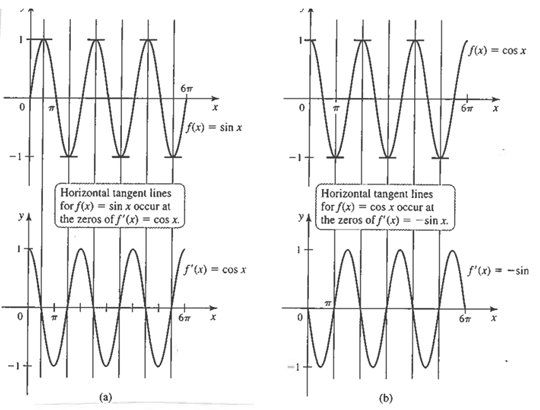
\includegraphics[scale=0.9]{pictures/Ch3sineCosine}
\end{center}
\end{frame}

% % %
\subsubsection{Trig Identities You Should Know}
% % %

% % %
\begin{frame}{\small Trig Identities You Should Know}
\begin{columns}[T]
\begin{column}{.5\textwidth}
\begin{itemize}\footnotesize
	\item $\sin^2 x + \cos^2 x = 1$ \vspace{0.2cm}
	\item $\tan^2 x + 1 = \sec^2 x$ \vspace{0.2cm}
	\item $\sin 2x =2\sin x \cos x$ \vspace{0.2cm}
	\item $\cos 2x = 1-2\sin^2 x$ \vspace{0.2cm}
	\item $\cos^2 x = \frac{1+\cos 2x}{2}$ \vspace{0.1cm}
	\item $\sin^2 x = \frac{1-\cos 2x}{2}$ \vspace{0.2cm}
\end{itemize}
\end{column}
\begin{column}{.5\textwidth}
\begin{itemize}\footnotesize
	\item $\tan x = \frac{\sin x}{\cos x}$ \vspace{0.2cm}
	\item $\cot x = \frac{\cos x}{\sin x}$ \vspace{0.2cm}
	\item $\cot x = \frac{1}{\tan x}$ \vspace{0.2cm}
	\item $\sec x = \frac{1}{\cos x}$ \vspace{0.1cm}
	\item $\csc x = \frac{1}{\sin x}$ \vspace{0.2cm}
\end{itemize}
\end{column}
\end{columns}
\end{frame}

% % %
\subsubsection{Derivatives of Other Trig Functions}
% % %

% % %
\begin{frame}{\small Derivatives of Other Trig functions}\footnotesize
\begin{align*}
\frac{d}{dx}(\tan x)&=\frac{d}{dx} \left( \frac{\sin x}{\cos x}\right) \\
 &= \frac{\cos x \cos x - (-\sin x)\sin x }{\cos^2 x} \\
&= \frac{\cos^2 x + \sin^2 x}{\cos^2 x} \\
&= \frac{1}{\cos^2 x} = \sec^2 x
\end{align*}
So \alert{$\frac{d}{dx} (\tan x)=\sec^2 x$}.
\end{frame}

% % %
\begin{frame}{}
By using trig identities and the Quotient Rule, we obtain
\begin{align*}
\alert{\frac{d}{dx} (\csc x)} &= \frac{d}{dx} \left( \frac{1}{\sin x}\right) = \alert{-\csc x \cot x} \\
\alert{\frac{d}{dx} (\sec x)} &= \frac{d}{dx} \left( \frac{1}{\cos x}\right) = \alert{\sec x \tan x} \\
\alert{\frac{d}{dx} (\cot x)} &= \frac{d}{dx} \left( \frac{1}{\tan x}\right) = \alert{-\csc^2 x}  
\end{align*}
\end{frame}

% % %
\begin{frame}
\begin{exe} Compute the derivative of the following functions:
\[f(x)=\frac{\tan x}{1+\tan x} \qquad g(x)=\sin x \cos x\]
\end{exe}
\end{frame}

% % %
\begin{frame}
\begin{exe} 
Use the difference and product rules to find the derivative of the function $y=\cos x-x\sin x$.
\begin{itemize}
\item[A. ] $-\sin x+x\cos x$
\item[B. ] $x\cos x$
\item[C. ] $-2\sin x-x\cos x$
\item[D. ] $x\cos x-2\sin x$
\end{itemize}
\end{exe}
\end{frame}

% % %
\subsubsection{Higher-Order Trig Derivatives}
% % %

% % %
\begin{frame}{\small Higher-Order Trig Derivatives}
There is a cyclic relationship between the higher order derivatives of $\sin x$ and $\cos x$:
\begin{columns}
\begin{column}{.45\textwidth}
\[\begin{split}
	f(x) &=\sin x \\  
	f^{\prime}(x) &=\cos x \\
	f^{\prime\prime}(x) &=-\sin x \\
	f^{(3)}(x) &=-\cos x \\
	f^{(4)}(x) &=\sin x 
\end{split}\]
\end{column}
\begin{column}{.6\textwidth}
\[\begin{split}
	g(x) &=\cos x \\
	g^{\prime}(x) &=-\sin x \\
	g^{\prime\prime}(x) &=-\cos x \\
	g^{(3)}(x) &=\sin x \\
	g^{(4)}(x) &=\cos x 
\end{split}\]
\end{column}
\end{columns}
\end{frame}

% % %
\subsubsection{Book Problems}
% % %

% % %
\begin{frame}
\begin{block}{3.5 Book Problems} 7-47 (odds), 57, 59, 61 \end{block} 
\end{frame}

% % %
\subsection[3.6 Derivatives as Rates of Change]{\S 3.6 Derivatives as Rates of Change}
% % %

% % %
\begin{frame}{\S 3.6 Derivatives as Rates of Change}
\begin{que}  
Why do we need derivatives in real life? 
\end{que}  

We look at four areas where the derivative assists us with determining the rate of change in various contexts.
\end{frame}

% % %
\subsubsection{Position and Velocity}
% % %

% % %
\begin{frame}{\small Position and Velocity}
Suppose an object moves along a straight line and its location at time $t$ is given by the position function $s=f(t)$.  The {\bf displacement} of the object between $t=a$ and $t=a+\Delta t$ is 
\[\Delta s = f(a+\Delta t)-f(a).\]
Here $\Delta t$ represents how much time has elapsed.
\end{frame}

% % %
\begin{frame}{}
We now define average velocity as 
\[\frac{\Delta s}{\Delta t}=\frac{f(a+\Delta t)-f(a)}{\Delta t}.\]
Recall that the limit of the average velocities as the time interval approaches 0 was the instantaneous velocity (which we denote here by $v$).  Therefore, the instantaneous velocity at $a$ is 
\[v(a)=\lim_{\Delta t \to 0} \frac{f(a+\Delta t)-f(a)}{\Delta t} = f^{\prime}(a).\]
\end{frame}

% % %
\subsubsection{Speed and Acceleration}
% % %

% % %
\begin{frame}{\small Speed and Acceleration}
In mathematics, speed and velocity are related but not the same -- if the \alert{velocity} of an object at any time $t$ is given by $v(t)$, then the \alert{speed} of the object at any time $t$ is given by 
\[|v(t)|=|f^{\prime}(t)|.\]
\end{frame}

% % %
\begin{frame}[allowframebreaks]{}
By definition, acceleration (denoted by $a$) is the instantaneous rate of change of the velocity of an object at time $t$.  Therefore,
\[a(t)=v^{\prime}(t)\]
and since velocity was the derivative of the position function $s=f(t)$, then 
\[a(t)=v^{\prime}(t)=f^{\prime\prime}(t).\]

\framebreak
{\bf Summary:}  Given the position function $s=f(t)$, the velocity at time $t$ is the first derivative, the speed at time $t$ is the absolute value of the first derivative, and the acceleration at time $t$ is the second derivative.
\end{frame}

% % %
\begin{frame}
\begin{que} Given the position function $s=f(t)$ of an object launched into the air, how would you know:
\begin{itemize}
	\item The highest point the object reaches?
	\item How long it takes to hit the ground?
	\item The speed at which the object hits the ground?
\end{itemize}
\end{que}
\end{frame}

% % %
\begin{frame}
\begin{exe}
A rock is dropped off a bridge and its distance $s$ (in feet) from the bridge after $t$ seconds is $s(t)=16t^2+4t$.  At $t=2$ what are, respectively, the velocity of the rock and the acceleration of the rock? 
\begin{itemize}
\item[A. ] $64$ ft/s; $16$ ft/s$^2$
\item[B. ] $68$ ft/s; $32$ ft/s$^2$
\item[C. ] $64$ ft/s; $32$ ft/s$^2$
\item[D. ] $68$ ft/s; $16$ ft/s$^2$
\end{itemize}
\end{exe}
\end{frame}

% % %
\subsubsection{Growth Models}
% % %

% % %
\begin{frame}{\small Growth Models}
Suppose $p=f(t)$ is a function of the growth of some quantity of interest.  The average growth rate of $p$ between times $t=a$ and a later time $t=a+\Delta t$ is the change in $p$ divided by the elapsed time $\Delta t$:
\[\frac{\Delta p}{\Delta t}=\frac{f(a+\Delta t)-f(a)}{\Delta t}.\]
\end{frame}

% % %
\begin{frame}{}
As $\Delta t$ approaches 0, the average growth rate approaches the derivative $\textstyle\frac{dp}{dt}$, which is the instantaneous growth rate (or just simply the growth rate).  Therefore,
\[\frac{dp}{dt}=\lim_{\Delta t \to 0} \frac{f(a+\Delta t)-f(a)}{\Delta t} = \lim_{\Delta t \to 0} \frac{\Delta p}{\Delta t}.\]
\end{frame}

% % %
\begin{frame}
\begin{exe} The population of the state of Georgia (in thousands) from 1995 ($t=0$) to 2005 ($t=10$) is modeled by the polynomial 
\[p(t)=-0.27t^2+101t+7055.\]
\begin{itemize}
	\item[(a)] What was the average growth rate from 1995 to 2005?
	\item[(b)] What was the growth rate for Georgia in 1997?
	\item[(c)] What can you say about the population growth rate in Georgia between 1995 and 2005?
\end{itemize}
\end{exe}
\end{frame}

% % %
\subsubsection{Average and Marginal Cost}
% % %

% % %
\begin{frame}{\small Average and Marginal Cost}
Suppose a company produces a large amount of a particular quantity.  Associated with manufacturing the quantity is a {\bf cost function} $C(x)$ that gives the cost of manufacturing $x$ items.  This cost may include a {\bf fixed cost} to get started as well as a {\bf unit cost} (or {\bf variable cost}) in producing one item.
\end{frame}

% % %
\begin{frame}{}
If a company produces $x$ items at a cost of $C(x)$, then the average cost is $\textstyle\frac{C(x)}{x}.$  This average cost indicates the cost of items already produced.  Having produced $x$ items, the cost of producing another $\Delta x$ items is $C(x+\Delta x)-C(x)$.  So the average cost of producing these extra $\Delta x$ items is 
\[\frac{\Delta C}{\Delta x}=\frac{C(x+\Delta x)-C(x)}{\Delta x}.\]
\end{frame}

% % %
\begin{frame}{}
If we let $\Delta x$ approach 0, we have
\[\lim_{\Delta x \to 0}\frac{\Delta C}{\Delta x}=C^{\prime}(x)\]
which is called the {\bf marginal cost}.  The marginal cost is the approximate cost to produce one additional item after producing $x$ items.

\vspace{1pc}
{\bf Note:}  In reality, we can't let $\Delta x$ approach 0 because $\Delta x$ represents whole numbers of items.
\end{frame}

% % %
\begin{frame}
\begin{exe} If the cost of producing $x$ items is given by 
\[C(x)=-0.04x^2+100x+800\]
for $0 \le x \le 1000$, find the average cost and marginal cost functions.  Also, determine the average and marginal cost when $x=500.$ \end{exe}
\end{frame}

% % %
\subsubsection{Book Problems}
% % %

% % %
\begin{frame}
\begin{block}{3.6 Book Problems} 9-19, 21-24, 30-33 (odds) \end{block}
\end{frame}

% % %
\subsection[3.7 The Chain Rule]{\S 3.7 The Chain Rule}
% % %

% % %
\begin{frame}{\S 3.7 The Chain Rule}\footnotesize
The rules up to now have not allowed us to differentiate composite functions 
\[
f\circ g(x)=f(g(x)).
\]
\begin{ex}
If $f(x)=x^7$ and $g(x)=2x-3$, then $f(g(x))=(2x-3)^7$.  To differentiate we could mulitply the polynomial out... but in general we should use a much more efficient strategy to emply to composition functions. 
\end{ex}
\end{frame}

% % %
\begin{frame}\footnotesize
\begin{ex}
Suppose that Yvonne ($y$) can run twice as fast as Uma ($u$). Then write $\textstyle\frac{dy}{du}=2$.

\vspace{0.5pc}
Suppose that Uma can run four times as fast as Xavier ($x$).  So $\textstyle\frac{du}{dx}=4$.

\vspace{1pc}
How much faster can Yvonne run than Xavier?  In this case, we would take both our rates and multiply them together:
\[\frac{dy}{du} \cdot \frac{du}{dx}=2 \cdot 4 = 8.\]
\end{ex}
\end{frame}

% % % 
\subsubsection{Version 1 of the Chain Rule}
% % %

% % %
\begin{frame}{\small Version 1 of the Chain Rule}
If $g$ is differentiable at $x$, and $y=f(u)$ is differentiable at $u=g(x)$, then the composite function $y=f(g(x))$ is differentiable at $x$, and its derivative can be expressed as 
\[\frac{dy}{dx}=\frac{dy}{du} \cdot \frac{du}{dx}\]
\end{frame}

% % %
\subsubsection{Guidelines for Using the Chain Rule}
% % %

% % %
\begin{frame}{\small Guidelines for Using the Chain Rule}\footnotesize
Assume the differentiable function $y=f(g(x))$ is given.
\begin{itemize}
	\item[1.] Identify the outer function $f$, the inner function $g$, and let $u=g(x).$
	\item[2.] Replace $g(x)$ by $u$ to express $y$ in terms of $u$:
	\[y=f(g(x)) \implies y=f(u)\]
	\item[3.]  Calculate the product $\frac{dy}{du} \cdot \frac{du}{dx}$
	\item[4.] Replace $u$ by $g(x)$ in $\frac{dy}{du}$ to obtain $\frac{dy}{dx}.$
\end{itemize}
\end{frame}

% % %
\begin{frame}\footnotesize
\begin{ex} Use Version 1 of the Chain Rule to calculate $\textstyle\frac{dy}{dx}$ for $y=(5x^2 +11x)^{20}$. \end{ex}
\begin{itemize}
\item inner function: $u=5x^2+11x$ 
\item outer function: $y=u^{20}$
\end{itemize}

\vspace{1pc}
We have $y = f(g(x)) = (5x^2 +11x)^{20}$.  Differentiate:
\begin{align*} 
\frac{dy}{dx}= \frac{dy}{du}\cdot\frac{du}{dx} &= 20u^{19} \cdot (10x+11) \\
 &=20(5x^2 +11x)^{19} \cdot (10x+11)
\end{align*}
\end{frame}

% % %
\begin{frame}
\begin{exe} Use the first version of the Chain Rule to calculate $\textstyle\frac{dy}{dx}$ for 
\[y=\left( \frac{3x}{4x+2} \right)^5.\]
\end{exe}
\end{frame}

% % %
\begin{frame}
\begin{exe}
Use the first version of the Chain Rule to calculate $\textstyle\frac{dy}{dx}$ for
\[
y=\cos{(5x+1).}
\]
\begin{itemize}
\item[A. ] $y'=-\cos{(5x+1)}\cdot\sin{(5x+1)}$
\item[B. ] $y'=-5\sin{(5x+1)}$
\item[C. ] $y'=5\cos{(5x+1)}-\sin{(5x+1)}$
\item[D. ] $y'=-\sin{(5x+1)}$
\end{itemize}
\end{exe}
\end{frame}

% % %
\subsubsection{Version 2 of the Chain Rule}
% % %

% % %
\begin{frame}{\small Version 2 of the Chain Rule}
Notice if $y=f(u)$ and $u=g(x)$, then $y=f(u)=f(g(x))$, so we can also write:
\begin{align*}
\frac{dy}{dx} &= \frac{dy}{du} \cdot \frac{du}{dx} \\[0.75pc]
 &= f^{\prime}(u) \cdot g^{\prime}(x) \\[0.75pc]
 &= f^{\prime}(g(x)) \cdot g^{\prime}(x).
\end{align*}
\end{frame}

% % %
\begin{frame}\footnotesize
\begin{ex} Use Version 2 of the Chain Rule to calculate $\textstyle\frac{dy}{dx}$ for $y=(7x^4+2x+5)^9$. \end{ex}
\begin{itemize}
\item inner function: $g(x)=7x^4+2x+5$ 
\item outer function: $f(u)=u^9$
\end{itemize}
Then
\begin{align*}
f^{\prime}(u) &= 9u^8 \implies f^{\prime}(g(x))=9(7x^4+2x+5)^8 \\
g^{\prime}(x) &=28x^3+2.
\end{align*}
Putting it together,
\[\frac{dy}{dx}=f^{\prime}(g(x)) \cdot g^{\prime}(x) = 9(7x^4+2x+5)^8 \cdot (28x^3+2)\]
\end{frame}

% % %
\begin{frame}
\begin{exe}
Use Version 2 of the Chain Rule to calculate $\textstyle\frac{dy}{dx}$ for
\[
y=\tan{(5x^5-7x^3+2x)}.
\]
\end{exe}
\end{frame}

% % %
\subsubsection{Chain Rule for Powers}
% % %

% % % 
\begin{frame}[allowframebreaks]{\small Chain Rule for Powers}
If $g$ is differentiable for all $x$ in the domain and $n$ is an integer, then
\[\frac{d}{dx} \bigg[\left(g(x)\right)^n \bigg]=n(g(x))^{n-1} \cdot g^{\prime}(x).\]

\framebreak
\begin{ex} $\frac{d}{dx} \bigg[ (1-e^x)^4 \bigg] =$ ? \end{ex}
{\bf Answer:}
\begin{align*}
\frac{d}{dx} \bigg[ (1-e^x)^4 \bigg] &= 4(1-e^x)^3 \cdot (-e^x) \\
 &= -4e^x (1-e^x)^3
\end{align*}
\end{frame}

% % %
\subsubsection{Composition of 3 or More Functions}
% % %

% % %
\begin{frame}[allowframebreaks]{\small Composition of 3 or More Functions}
\begin{ex}Compute $\frac{d}{dx} \bigg[ \sqrt{(3x-4)^2 + 3x} \bigg]$. \end{ex}

\framebreak\footnotesize
{\bf Answer:}
\begin{alignat*}{2}
\frac{d}{dx} \bigg[ \sqrt{(3x-4)^2 + 3x} \bigg] &= \frac{1}{2} \big( (3x-4)^2 + 3x \big)^{-\frac{1}{2}} \cdot \frac{d}{dx} \big[ (3x-4)^2 + 3x \big] \\
&= \frac{1}{2 \sqrt{ \big( (3x-4)^2 + 3x \big)}} \cdot \bigg[ 2(3x-4) \frac{d}{dx}(3x-4)  + 3 \bigg] \\
&= \frac{1}{2 \sqrt{ \big( (3x-4)^2 + 3x \big)}} \cdot \big[ 2(3x-4) \cdot 3 + 3 \big] \\
&= \frac{18x-21}{2 \sqrt{ \big( (3x-4)^2 + 3x \big)}} 
\end{alignat*}
\end{frame}

% % %
\subsubsection{Book Problems}
% % %

% % %
\begin{frame}
\begin{block}{3.7 Book Problems} 7-33 (odds), 38, 45-67 (odds) \end{block} 
\end{frame}

% % %
\subsection[3.8 Implicit Differentiation]{\S 3.8 Implicit Differentiation}
% % %

% % %
\begin{frame}{\S 3.8 Implicit Differentiation}\footnotesize
Up to now, we have calculated derivatives of functions of the form $y=f(x)$, where $y$ is defined {\bf explicitly} in terms of $x$.  In this section, we examine relationships between variables that are {\bf implicit} in nature, meaning that $y$ either is not defined explicitly in terms of $x$ or cannot be easily manipulated to solve for $y$ in terms of $x$.

\vspace{1pc}
The goal of {\bf implicit differentiation} is to find a single expression for the derivative directly from an equation of the form $F(x,y)=0$ without first solving for $y$.
\end{frame}

% % %
\begin{frame}{}
\begin{ex} Calculate $\textstyle\frac{dy}{dx}$ directly from the equation for the circle 
\[x^2 + y^2 = 9.\]
\end{ex}
{\bf Solution:}  To remind ourselves that $x$ is our independent variable and that we are differentiating with respect to $x$, we can replace $y$ with $y(x)$:
\[x^2 + (y(x))^2 = 9.\]
\end{frame}

% % %
\begin{frame}\footnotesize
Now differentiate each term with respect to $x$:
\[\frac{d}{dx} (x^2) + \frac{d}{dx} ((y(x))^2) = \frac{d}{dx}(9).\]
By the Chain Rule, $\textstyle\frac{d}{dx}((y(x))^2)=2y(x) y^{\prime}(x)$ (Version 2), or $\textstyle\frac{d}{dx}(y^2)=2y \frac{dy}{dx}$ (Version 1).  So 
\begin{align*}
2x+2y \frac{dy}{dx} &= 0 \\
\implies \alert{\frac{dy}{dx}} &= \frac{-2x}{2y} \\
	&= \alert{-\frac{x}{y}}.
\end{align*}
\end{frame}

% % %
\begin{frame}\footnotesize
The derivative is a function of $x$ and $y$, meaning we can write it in the form 
\[F(x,y)=-\frac{x}{y}.\] 
To find slopes of tangent lines at various points along the circle we just plug in the coordinates.  For example, the slope of the tangent line at (0,3) is 
\[\left. \frac{dy}{dx} \right|_{(x,y)=(0,3)} = -\frac{0}{3}=0.\]
The slope of the tangent line at $(1,2\sqrt{2})$ is
\[\left. \frac{dy}{dx} \right|_{(x,y)=(1,2\sqrt{2})} = -\frac{1}{2\sqrt{2}}.\]
\end{frame}

% % %
\begin{frame}\footnotesize
The point is that, in some cases it is difficult to solve an implicit equation in terms of $y$ and then differentiate with respect to $x$.  In other cases, although it may be easier to solve for $y$ in terms of $x$, you may need two or more functions to do so, which means two or more derivatives must be calculated (e.g., circles).

\vspace{1pc}
The goal of implicit differentiation is to find one single expression for the derivative directly given $F(x,y)=0$ (i.e., some equation with $x$s and $y$s in it), without solving first for $y$.
\end{frame}

% % %
\begin{frame}%{\small Examples of functions implicitly defined}
\begin{que} The following functions are \alert{implicitly} defined:
\begin{itemize}
\item $x+y^3-xy=4$
\item $\cos(x-y)+\sin y = \sqrt{2}$
\end{itemize}
For each of these functions, how would you find $\textstyle\frac{dy}{dx}$?
\end{que}
\end{frame}

% % %
\begin{frame}{}
\begin{exe} Find $\textstyle\frac{dy}{dx}$ for $xy+y^3=1$. \end{exe}
\begin{exe} Find an equation of the line tangent to the curve $x^4-x^2 y+y^4=1$ at the point $(-1,1)$. \end{exe}
\end{frame}

% % %
\subsubsection{Higher Order Derivatives}
% % %

% % %
\begin{frame}{\small Higher Order Derivatives}
\begin{ex} Find $\textstyle\frac{d^2 y}{dx^2}$ if $xy+y^3=1$. \end{ex}
\end{frame}

% % %
\begin{frame}
\begin{exe}
If $\sin x=\sin y$, then $\textstyle\frac{dy}{dx}=$\ ? and $\textstyle\frac{d^2y}{dx^2}=$\ ?
\begin{itemize}
\item[A. ]$\frac{\cos y}{\cos x};\quad \frac{\tan y\cos^2x-\sin x\cos y}{\cos^2x}$
\item[B. ]$\frac{\cos x}{\cos y};\quad \frac{\tan y\cos^2x-\sin x\cos y}{\cos^2y}$
\item[C. ]$\frac{\cos x}{\cos y};\quad \frac{\cos y(\sin x-\sin y)}{\cos^2 y}$
\item[D. ]$\frac{\cos y}{\cos x};\quad \frac{\cos y(\sin x-\sin y)}{\cos^2 x}$
\end{itemize}
\end{exe}
\end{frame}

% % %
\subsubsection{Power Rule for Rational Exponents}
% % %

% % %
\begin{frame}{\small Power Rule for Rational Exponents}
Implicit differentiation also allows us to extend the power rule to rational exponents:  Assume $p$ and $q$ are integers with $q \neq 0$.  Then 
\[\alert{\frac{d}{dx} (x^{\frac{p}{q}})=\frac{p}{q} x^{\frac{p}{q}-1}}\]
(provided $x \geq 0$ when $q$ is even and $\textstyle\frac{p}{q}$ is in lowest terms).
\begin{exe}Prove it. \end{exe}
\end{frame}

% % %
\subsubsection{Book Problems}
% % %

% % %
\begin{frame}
\begin{block}{3.8 Book Problems} 5-25 (odds), 31-49 (odds) \end{block} 
\end{frame}

\end{document}